\documentclass[10pt,letterpaper]{article}
\usepackage{amsmath}
\usepackage{amsfonts}
\usepackage{amssymb}
\usepackage[english]{babel}
\usepackage{breakurl}
\usepackage[superscript]{cite}
\usepackage{draftwatermark}
\usepackage{fancyhdr}
\usepackage{float}
\usepackage[margin=1in]{geometry}
\usepackage{graphicx}
\usepackage{hyperref}
\usepackage[utf8]{inputenc}
\usepackage{makeidx}
\usepackage{multicol}
\usepackage{nth}
% \usepackage[default,scale=1.0]{opensans}
\usepackage{setspace}
\usepackage{siunitx}
\usepackage{svg}
\usepackage{subcaption}
\usepackage{tikz}
\usepackage{url}
\usepackage{kantlipsum}

%% Preamble
% Custom commands
\newcommand{\ts}{\textsubscript}

% Use hyphans to break up urls
\def\UrlBreaks{\do\/\do-}

% Draft watermark
\SetWatermarkText{\textsc{Draft}}
\SetWatermarkScale{5}

% PDF and href setup
% Hyper ref
\hypersetup{
	colorlinks=true,
	citecolor=black,
	linkcolor=black,
	filecolor=black,
	urlcolor=blue,
	pdftitle={Engineering Economic Analysis Report of Renewable Technologies},
	bookmarks=true
}
\urlstyle{same}

% Page semantics
\pagestyle{fancy}
\fancyhead[L]{\slshape\MakeUppercase{MECH 431}}
\fancyhead[R]{\slshape Muchen He}
\fancyfoot{}
\fancyfoot[C]{\thepage}

\parindent 0ex

% Meta
\author{Muchen He}
\title{Renewable Energy For Average Household in Edmonton}
\begin{document}
\begin{titlepage}
	\begin{center}
		Draft build 121\\
		\vspace*{3in}
		\line(1, 0){400}\\
		\Huge{\textbf{Renewable Energy For An Average Household in Edmonton}}\\[0.2cm]
		\large{\textbf{Engineering Economic Analysis Report of Renewable Technologies}}\\[1cm]
		\Large{\textbf{MECH 431}}\\
		\textbf{University of British Columbia}\\
		\line(1, 0){400}\\
		\vfill
		\Large{Muchen He}\\
		44638154\\

		\today\\
	\end{center}
\end{titlepage}

% Table of contents
\setcounter{secnumdepth}{3}
\tableofcontents
\thispagestyle{empty}
\clearpage

% Uncomment for list of tables and figures
\thispagestyle{empty}
\listoffigures
\listoftables
\newpage

% Set page and section counter
\setcounter{page}{1}

\section{Introduction}\label{section:introduction}

\subsection{Problem}

Edmonton, being the "Oil city", the captial of the province whose major export is oil, is relying too much on non-renewanle resources like fossil fuel. Thus we need to take steps to move towards greener solutions.\\

% TODO:
Edmonton average household consumes <INSERT> megawatts per year. It would be world changing if all these electrical energy can be derived from renewable sources.\\
\\
Alberta consumes more than 10,000 GWh of energy a year. This averages to about 2400 kWh per capita\cite{average-albertan-consumption}. The province has an over-reliance on non-renewable resources for its power generation. Furthermore, projects involving building pipelines and method of hydraulic fracturing (fracking) poses serious environmental impact\cite{fracking-kurzgesagt}.
\\
This report intends to explore the economic viablility of renewable solutions that an individual or a family can realistically implement.\\
\\

\subsection{Solution Overview}

To solve this problem, we will look at the economic analysis of solar solutions. The analysis outlines the economic criteria and economic viability of implementing solar generation for a single average household in the sub-urban neighbourhoods of Edmonton.\\
\\
An adequate sustainable solar system should take pressure off of drawing energy from the grid, the electric companies, whose energy is generated from natural gas, coal, and oil. There are three main parts:

% TODO: change this to ordered list
\begin{itemize}
	\item Generation
	\item Storage
	\item Utilization
\end{itemize}

\section{Design}

The designs will be based on a template, and the template is derived from my house, which is an average Edmontonian house in the sub-urban neighbourhood of Terwillegar. This type of landscape and house is ubiquitous throughout Edmonton and thus would make an adequate model.\\

\begin{figure}[H]
	\centering
	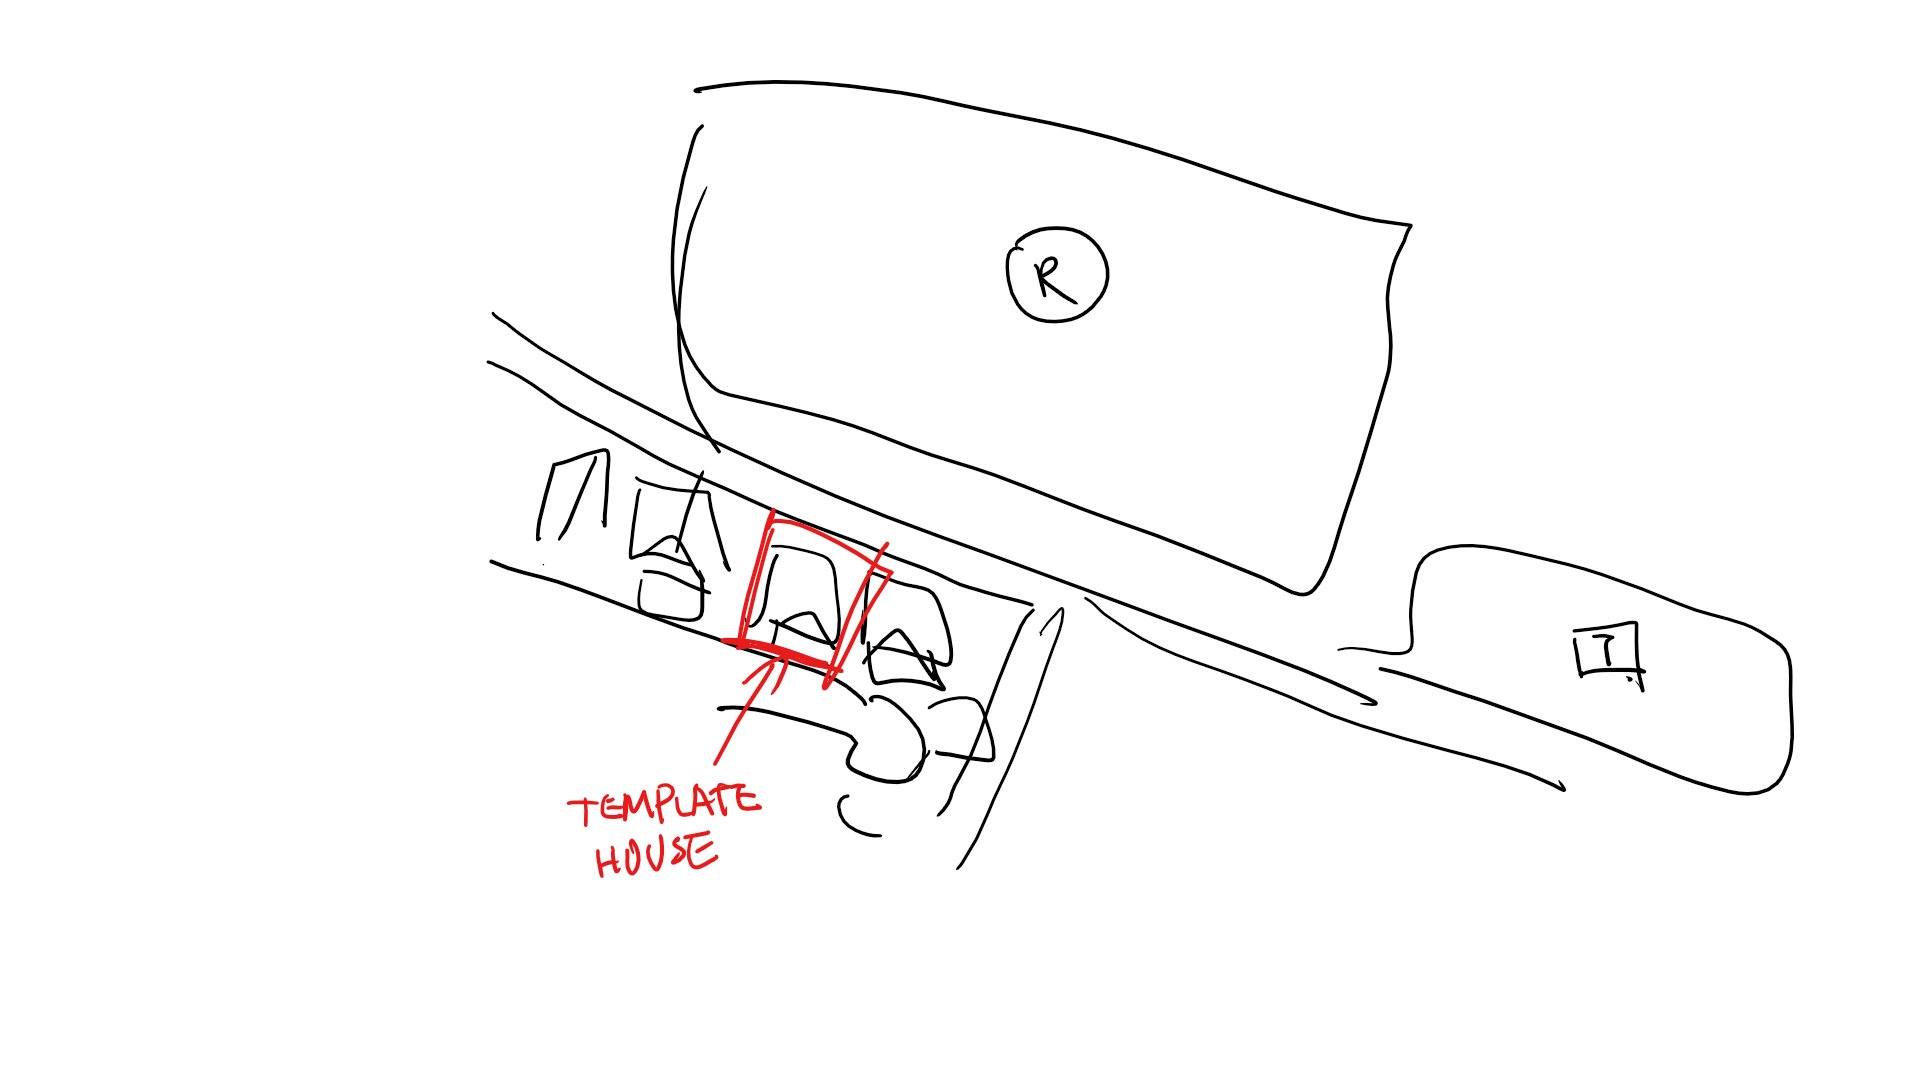
\includegraphics[width=0.6\textwidth]{assets/template-house-map}
	\caption{Map of the template house and its relative layout to the neighbourhood}
	\label{fig:template-house-path}
\end{figure}


\subsection{RCGs}\label{subsection:rcgs}
We will consider the requirement, constraints, and goals (RCGs) of the the project design which will be factors used to evaluate the successfulness of the project.

\subsubsection{Requirements}

The requirement is the criteria that determines if the project is a success or fail. The alternatives and layouts we consider should all meet the requirements.\\
\\
\textbf{Power Usage}
The average power generated must meet the average daytime usage. Data shows that the average Canadian household uses 11,135 kWh of electricity in the year 2014. In Alberta, the electricity usage is 7,200 kWh because there are more natural gas usage that offsets the electricity use. In fact, 77\% of total energy consumption (including electricity generation) is by natural gas. Ontario households uses 9,500 kWh per year.\cite{residential-energy-use}\\
\\
It's also worth noting that in a family of four, assuming 118 hours of hot water use, 415 kWh is used for water heaters. There are abundant solar powered water heaters on the market (very popular in developing countries including China). The government of Canada recommends weather-proof year round solar domestic hot water (SDHW) systems. \cite{residential-energy-use, gc-solar-water-heater}.\\
\\
Finding the daily average, the daily energy use is given by
$$
E_\text{daily}=7200\times10^3\div 365.25 = 19.7\text{kWh per day}
$$
A completely sustainable system would need to supply an at least 19.7kWh per day, or 821.36 Watts. But that is assuming a constant uniform use of 821.36W for 24 hours. So we can build a model where we assume no electricity is used overnight, or a model that realistically reflects the activity (shown below in figure \ref{fig:power-use-day}). The battery should have an output of at least 1.6kW during high-demand.
\\
\begin{figure}[H]
	\centering
	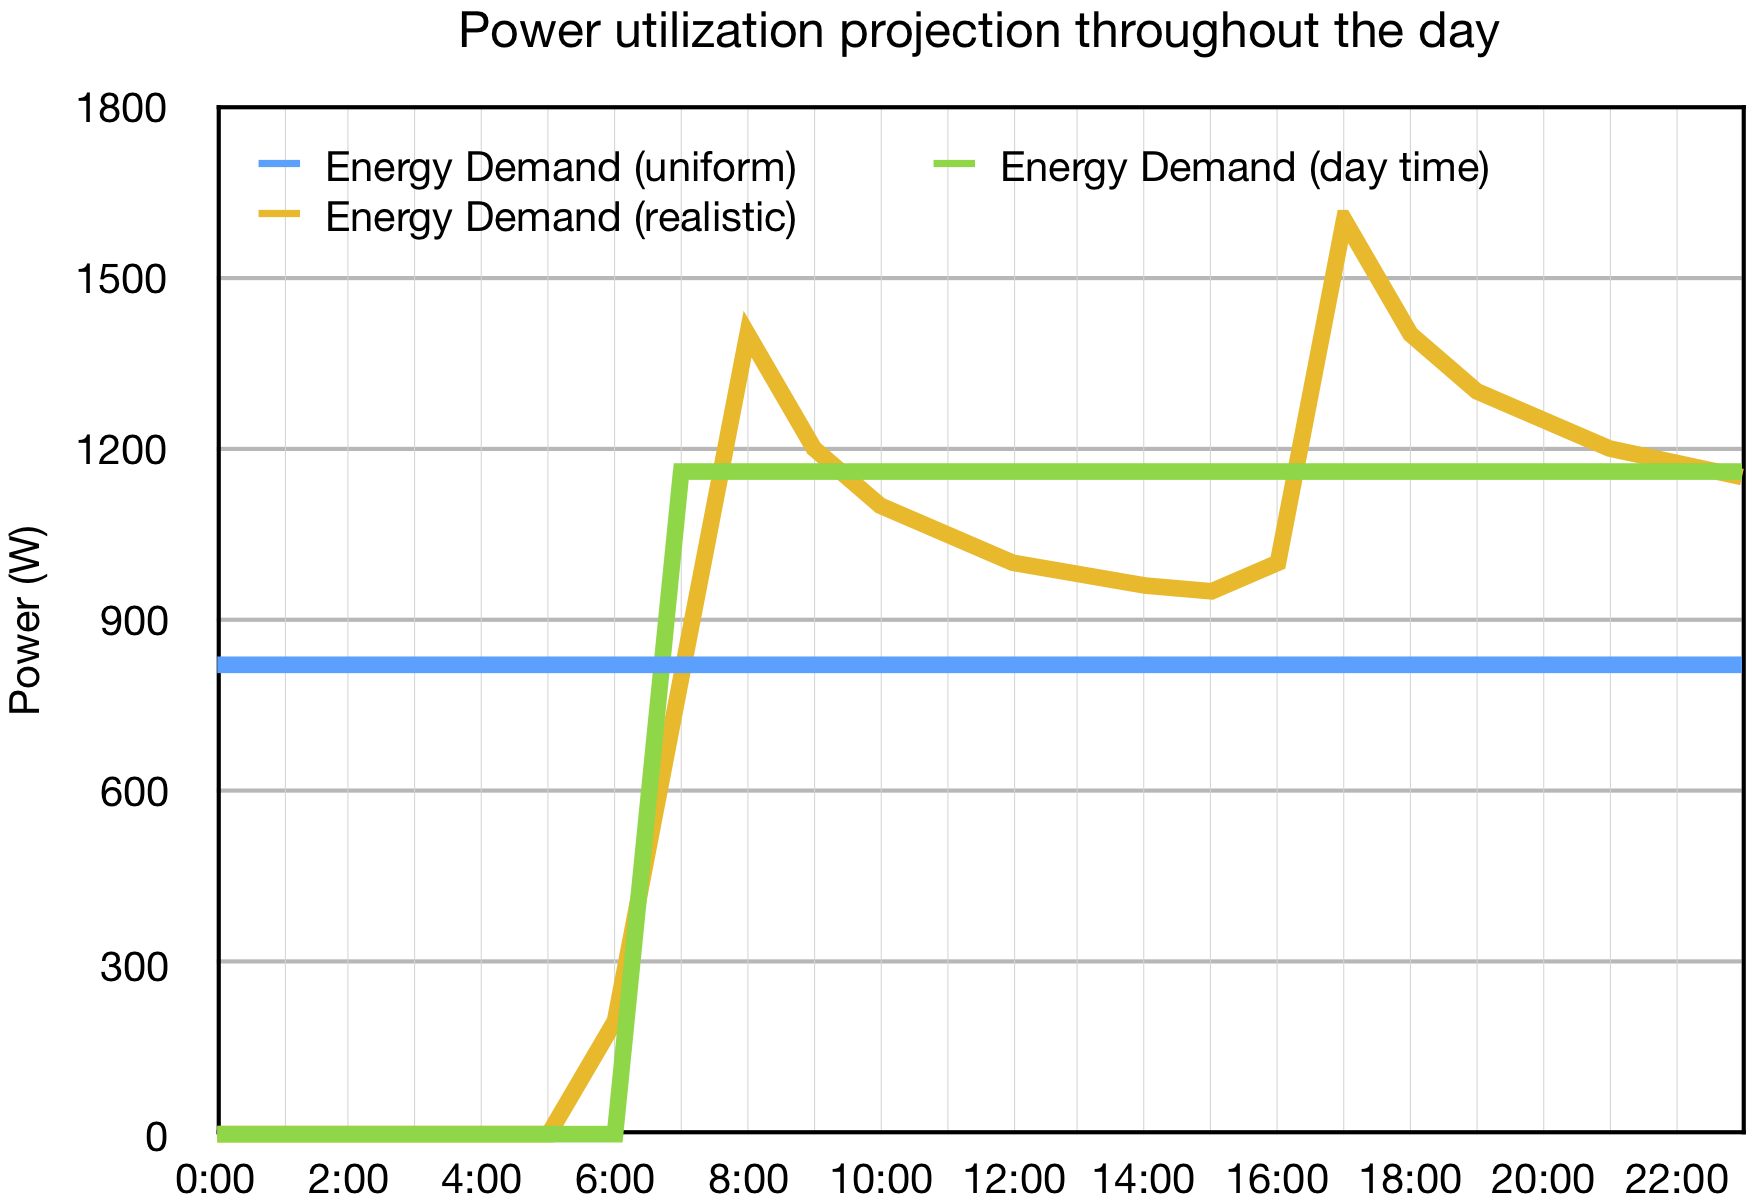
\includegraphics[width=0.6\textwidth]{assets/power-use-day}
	\caption{Average projected power use throughout 24 hours}
	\label{fig:power-use-day}
\end{figure}

\textbf{Reliability}\\
In the best case, the sun rises at 6:00, and sets at 20:00. Which means in the morning we need to have some reserve energy stored in the battery from 20:00 to midnight to next morning 6:00 (based off of figure \ref{fig:power-use-day}).\\
\\
\textbf{Rate of Return}\\
The rate of return should be greater than 2\%. Because 2\% is at least the inflation rate if the money is not put to use. (Additional MARR may apply if we take out loans to cover the cost of the project).

\subsubsection{Constraints}

The constraints are what the design is limited to, as well as any economic challenges and limits.\\
\\
Note that there is no contrainted on the input of the ecnomic model (capital is not fixed) and there is no constraints on the output of the economic model (power generated is not fixed, because extra power could be stored or sold).
\\
If the system is not able to achive the power demanded, the extra power will be drawn from power companies. Thus a negative cashflow is incurred from the money saved (if any). The opposite is true that extra power that can't be used or saved locally can be sold to power companies or re-channeled to neighbouring houses where there is more demand.\\

\subsubsection{Goals}

The goals for this project are the additional benefits that are optional to achieve, but the more the better.\\
\\
The MARR would be flexible if we're proceeding this project by using my own (or family's) money or savings to pay for the costs.

\subsection{Type}

What type of solar panels do we want to go for? The prominent three options available are:

\textbf{Form-Factor}
The form factor will determine how they will get installed, and roof area coverage efficiency. They also contribute to mainenance costs.\\
\begin{itemize}
	\item Traditional solar panels with reinforced glass and metal frames
	\item SolarCity solar shingles or equivalent
\end{itemize}

Once we determined the form factor, there are four types of solar cells, each with different efficiency and cost. For some solar cells, extra equipment and prerequisits are required.\\
\\
TODO: fix formatting of this table.\\
\begin{table}[H]
	\begin{tabular}{ |c|c|c|c| }
		\hline\\
		Solar Cell Type & Efficiency-Rate &Advantages &Disadvantages\\

		\hline\\
		
		Monocrystalline Solar Panels (Mono-SI)&~20\%&High efficiency rate; optimised for commercial use; high life-time value &Expensive\\

		\hline\\
		
		Polycrystalline Solar Panels (p-Si)&~15\%&Lower priceSensitive to high temperatures; lower lifespan & slightly less space efficiency\\
		\hline\\
		
		Thin-Film: Amorphous Silicon Solar Panels (A-SI)&~7-10\%&Relatively low costs; easy to produce \& flexible&shorter warranties \& lifespan\\

		\hline\\

		Concentrated PV Cell (CVP)&~41\%&Very high performance \& efficiency rate&Solar tracker \& cooling system needed (to reach high efficiency rate)\\

		\hline
	\end{tabular}
	\caption{Different types of solar cells and their advantages and disadvantages\cite{solar-panel-types}}
\end{table}

\subsection{Cooling}

For certain type of solar panels, overheating causes serious performance issues. Thus, cooling (extra non-recurring cost for installation, and recurring cost of maintainence) is required.\cite{pv-solar-cooling}\\

\subsection{Location}
Available location is located on the front, left and right slopes of the roof. With the front facing south (most direct sunlight).\\
\\
The output power of the solar panel is proportional to the strength of the sunlight received. The strength 

\subsection{Battery}

The battery is as critical as the solar panel itself as it's needed for a rainy day (pun intended). During higher peaks or at night, the solar panel will be unable to provide enough electrical power and thus a fall-back such as a battery or generator is required. Since we are only considering renewable energy, generators will be excluded.\\
\\
The most popular option is the Tesla Powerwall\cite{tesla-powerwall}. Tesla's website gives the option to select 1-10 power walls. These batteries will cost 8,100 USD per unit with a 960 USD price tag on supporting hardware (regardless of how many units).\\
\\
Assuming daily consumption of 20kWh per day, a single Poweerwall unit can deliver for 12 hours.\\

\subsection{Other equipment}

An inverter is required to generate usable sine-wave for AC applications.\\
\\
Technlogies may also be applied on the \textit{consuming} end. These include tools or gadgets that incur an initial cost, but have a small impact in reducing electricity use.\\
\\
Power factor correction can also reduce electric bills in case that we do need to tap power from utility companies.\\

\section{Paramters for Alternatives}\label{section:parameters}

This section compiles all conditions from previous section into a list of parameters that we wish to choose for our alternatives.\\

\subsection{Solar Panels}

\begin{itemize}
	\item Grape Solar 300W Monocrystalline Kit [\$2400]: provides approx. 900Wh of energy; it has 3 panels (48"x22") and comes with an inverter\cite{hd-solar1}.

	\item Canadian Solar – 325W polycrystalline module [\$270]\cite{raysolar-solar1}

	\item Heliene 160W Monocrystalline PV module [\$295] \cite{raysolar-solar2}
\end{itemize}

\subsection{Mounting}

\subsection{Battery}

\subsection{Inverter}

\subsection{Electronics}

\section{Alternatives}

TODO:\\
\\
Here I will select a few alternatives given by choosing the parameters outlined in the previous section (section \ref{section:parameters}) and use them as possible alternatives. The do-nothing alternative is implied by selecting 0 solar panels, 0 batteries, and no auxillery upgrades.\\

\section{Economic Model}
As briefed explained in section \ref{subsection:rcgs}, the economic model will be a combination of segmenting model, where the cashflows are broken into differet core components, learning curve model (for modelling the effective of technlogy and repetitive installation). Finally, the cost index model for market prices of products.\\

\subsection{Expected Cashflow-In}
The main benefit or positive cashflow is from the savings in electrical bills. We would also need to analyze the current and projected future cost to electricty from utility companies. Note that electricity costs may even change throughout the year as demand changes.\\
\\
There are various other ways that would invoke a positive cash flow:\\

\begin{itemize}
	\item Alberta government incentives that promotes green energy; they provide a fixed cash-back from receipts of purchases of renewable technologies. This will be a one-time / non-recurring benefit.

	\item Extra, unused power may be sold back to utility companies; they could also be redirected to other households whose demands are higher.

	\item Salvage value for the technologies and equipment at the end of analysis period. If well-maintained, there should be a high resale value as demand for renewable equiment increases in time.
\end{itemize}

\subsection{Expected Cashflow-Out}\label{subsection:cashflow-out}

We should expect majority of the cost will be the initial cost of equipment and installation.\\
\\
If the solar panels or installation is financed, then the initial cost would be the down-payment. However, we would also expect a debt with interest $i$. This will ultimately affect our MARR in our rate of return analysis (section \ref{subsection:rate-of-return}).\\
\\
Post-installation, there will be periodic cost to maintain the equipment. The solar panels would only need to be cleaned, and replacement is only necessary when the cells fail, which has low probability. Another periodic cost would be replacement of the batteries. Eventhough the batteries are rechargeable, they have about 5,000 full charge cycles while their effective performance and capacity decrease over time\cite{tesla-powerwall-wiki}.\\

\subsection{Sources of Capital}

For minimum risk in rate or return, all funding will come from other family members taking dividends in the project. The source of capital will be our savings and income.\\
\\
Alternatively, to put on less pressure financially in present time, we could choose to take out a one-time loan to pay all project costs up-front. The interest rate $i$ of the loan will mostly drive the MARR in the rate of return analysis (section \ref{subsection:rate-of-return}).\\
\\
Lastly, we could choose not to take loan, but finance the cost to install assuming that such option is available. Again, as mentioned in section \ref{subsection:cashflow-out}, the interest rate of the financing plan will affect the MARR.\\

\subsection{Taxes}
\begin{center}
	This section is intentionally left blank (haven't covered there in the course yet).\\
\end{center}

\section{Analysis}

We will run the analysis period for three time-scales: 

\begin{itemize}
	\item short-term (5 years) - appropriate for if we don't stay at the house very long (such as for when the house gets sold or rented out). Since 5 years is short, it's likely that the equipment and technology are not yet obsolete. Thus for this analysis period, we would account for the extra salvage value / resale value at the end of the 5 year period.\\

	\item medium-term (20 years) - this is the most realistic time period for most home-owners. The projection of power company electricity costs will be estimated using cost-index. The improvement in technlogy for the replaced solar panels are modelled as learning curve model.\\

	\item long-term (40 years) - this analysis period is appropriate for long term residency. The market price, cost index, and technology efficiency would be quite inaccurate in the far future. The assumption is that we would still be using the same system.
\end{itemize}

\subsection{Net Present Value Analysis}

For each of the three analysis periods, a net present value analysis will be performed. The assumption is that everything is re-purchaseable. The cost of replacement will follow a model based on the cost index trends.\\
\\
The NPV should infer roughly a good solution.\\
\\

\subsection{Equivalent Annual Cashflow Analysis}
The different alternatives would have different lifetimes and replacement would be required. We will consider \textbf{Replacement analysis}. When the old panel become so inefficient that the equivalent annual cost to operate the old panel (including the extra cost paid to the power companies) is greater than the equivalent annual cost of buying and operating new panels.\\

\subsection{Rate of Return Analysis}\label{subsection:rate-of-return}
Here we will compute the IRR of the given alternatives for all three analysis periods.\\

\section{Simulation}

The simulation will run for all three proposed analysis periods. For the 5 year perio, historical weather data will be collected and ran through the simulation. For 20 and 40 years, based on historical data, random weather conditions will be generated.\\
\\
These simulations will serve as a resiliency test, and the final cost at the end of the simulation period will be compared amongst the alternatives.\\

\section{Sensitivity and Risk Analysis}

After initial simulation, individual parameters such as compass-heading of the house, climate conditions, etc. will be altered to the simulation. This will yield how much the NPV or ECAF will change with respect to these alterations.\\

\section{Non-Economic Factors}
\subsection{Challenges}
- Alberta population's main economic driver is still fossil fuel, the public perception and public interst is not as sustainable as we preferred. This leads to lower supply of sustainable technlogies such as solar panels which drives up the price.\\

\section{Conclusion}\label{section:conclusion}

\subsection{Verdict}

% Bibliography
\clearpage
\addcontentsline{toc}{section}{References}
\bibliographystyle{ieeetr}
\bibliography{references}

\end{document}